% Ubah judul dan label berikut sesuai dengan yang diinginkan.
\section{Result}
\label{sec:results}
 
The metrics employed to assess the efficacy of the model during training are accuracy and loss. These two metrics are utilized to ascertain the suitability of the model for the task at hand. However, they may prove challenging in predicting data that has never been encountered by the model.

The testing process involves three models, namely the model with the highest training accuracy value, the model with the highest validation value, and the last model in training.

The results of this study were evaluated using several additional metrics, including precision, recall, and F1-score. These metrics are employed to assess the accuracy of the model that has been developed.
\subsection{Model Testing Results Without Using class-weight Adjustment}
\begin{figure}[H]
	\centering
	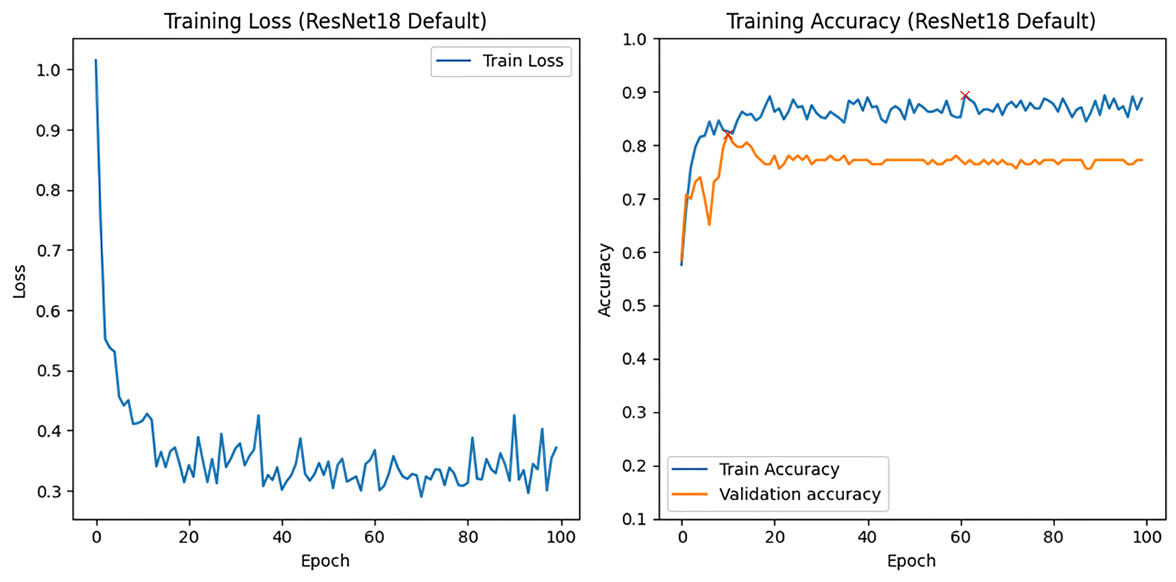
\includegraphics[height=4cm]{gambar/TrainingGraphResNet18.png}
	\caption{Graph of Training Loss and Accuracy from ResNet-18 Without Class-weight Adjustment}
	\label{Fig:GraphTrainingDefPt1}
\end{figure}
\begin{figure}[H]
	{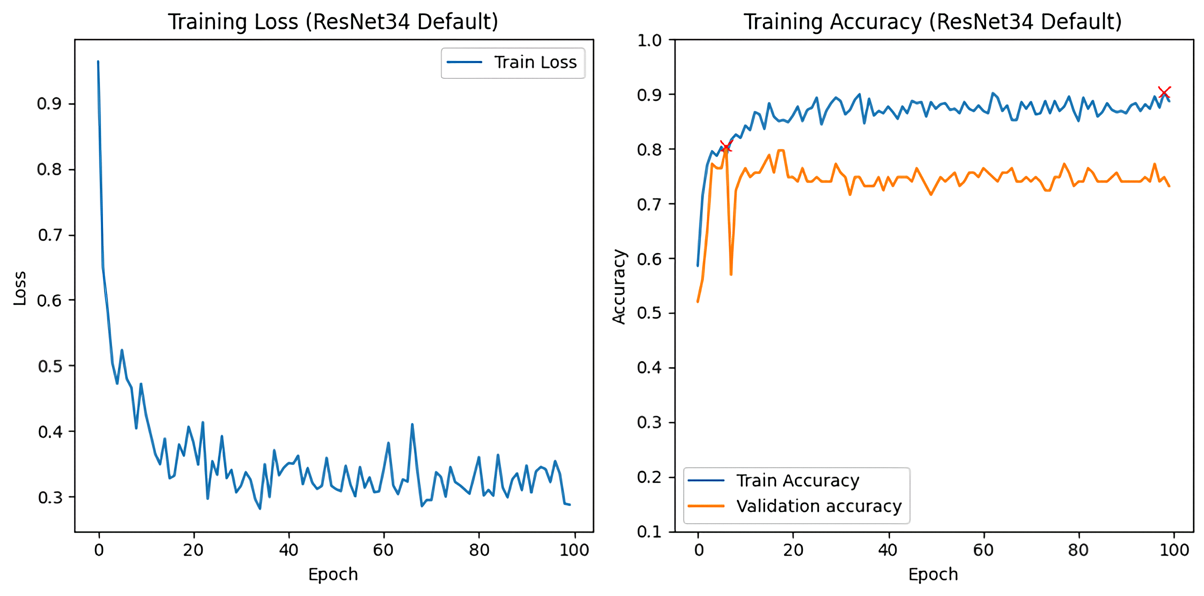
\includegraphics[height=4cm]{gambar/TrainingGraphResNet34.png}}
	\caption{Graph of Training Loss and Accuracy from ResNet-34 Without Class-weight Adjustment}
	\label{Fig:GraphTrainingDefPt2}
\end{figure}
\begin{figure}[H]
	\centering
	{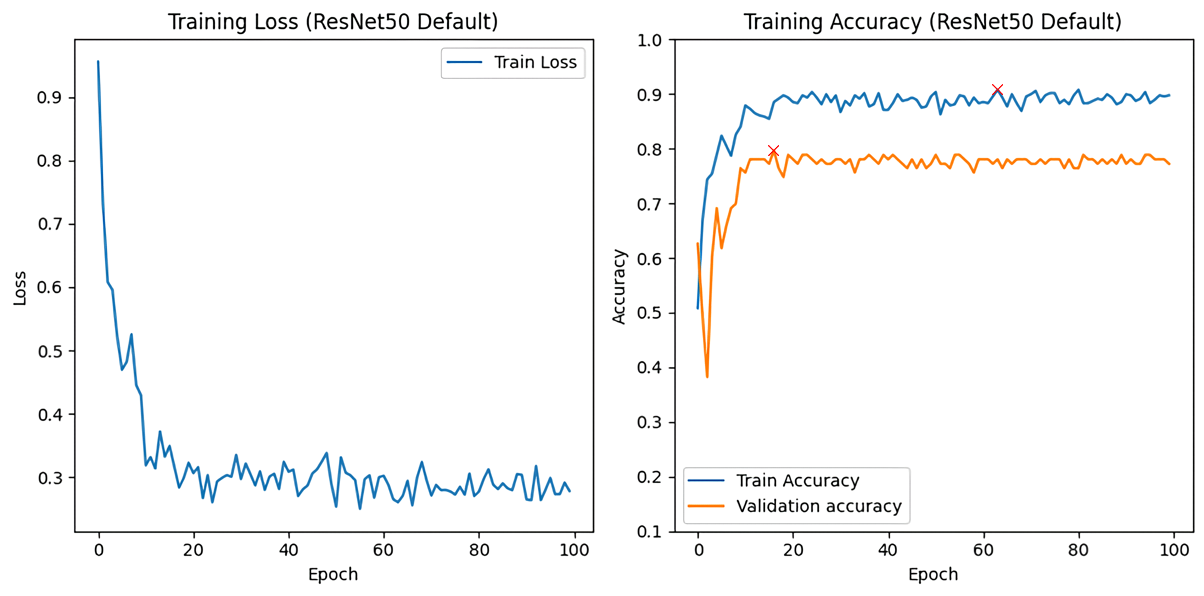
\includegraphics[height=4cm]{gambar/TrainingGraphResNet50.png}}
	\caption{Graph of Training Loss and Accuracy from ResNet-50 Without Class-weight Adjustment}
	\label{Fig:GraphTrainingDefPt3}
\end{figure}
\begin{figure}[H]
	{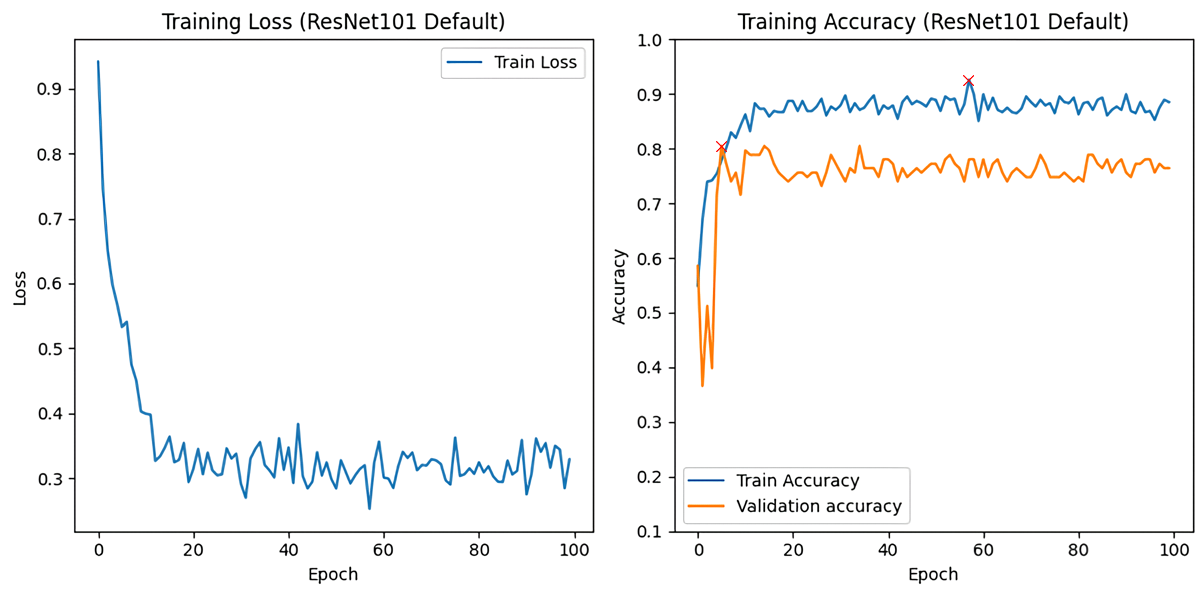
\includegraphics[height=4cm]{gambar/TrainingGraphResNet101.png}}
	\caption{Graph of Training Loss and Accuracy from ResNet-101 Without Class-weight Adjustment}
	\label{Fig:GraphTrainingDefPt4}
\end{figure}
\begin{figure}[H]
	{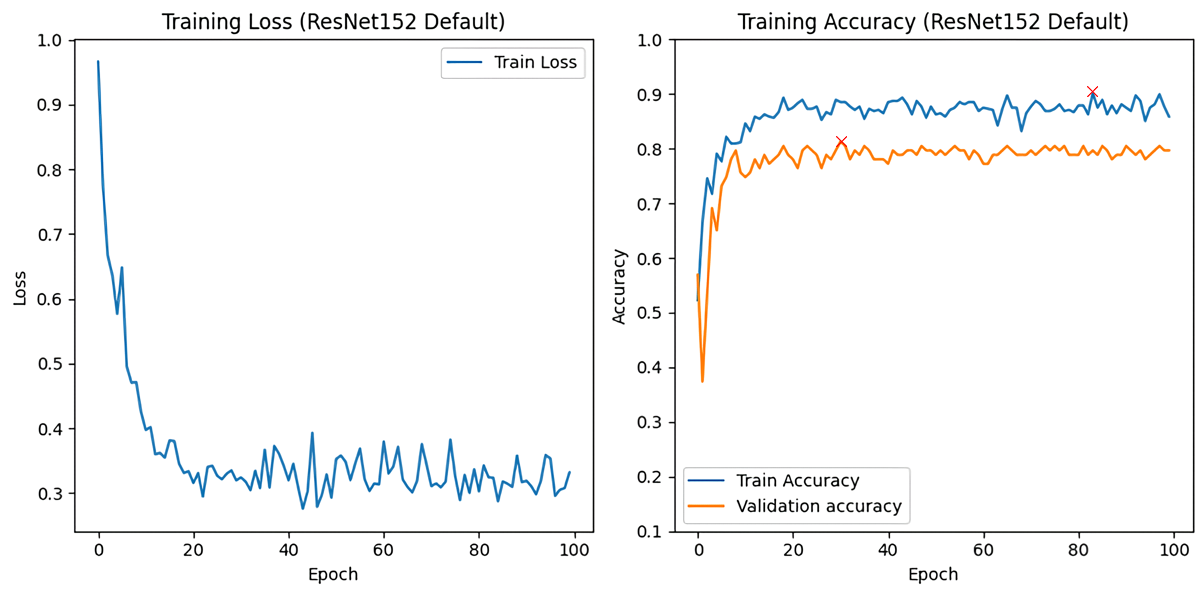
\includegraphics[height=4cm]{gambar/TrainingGraphResNet152.png}}
	\caption{Graph of Training Loss and Accuracy from ResNet-152 Without Class-weight Adjustment}
	\label{Fig:GraphTrainingDefPt5}
\end{figure}

\subsection{Model Testing Results Using class-weight Adjustment}
\label{sec:412}
\begin{figure}[hbtp]
	\centering
	{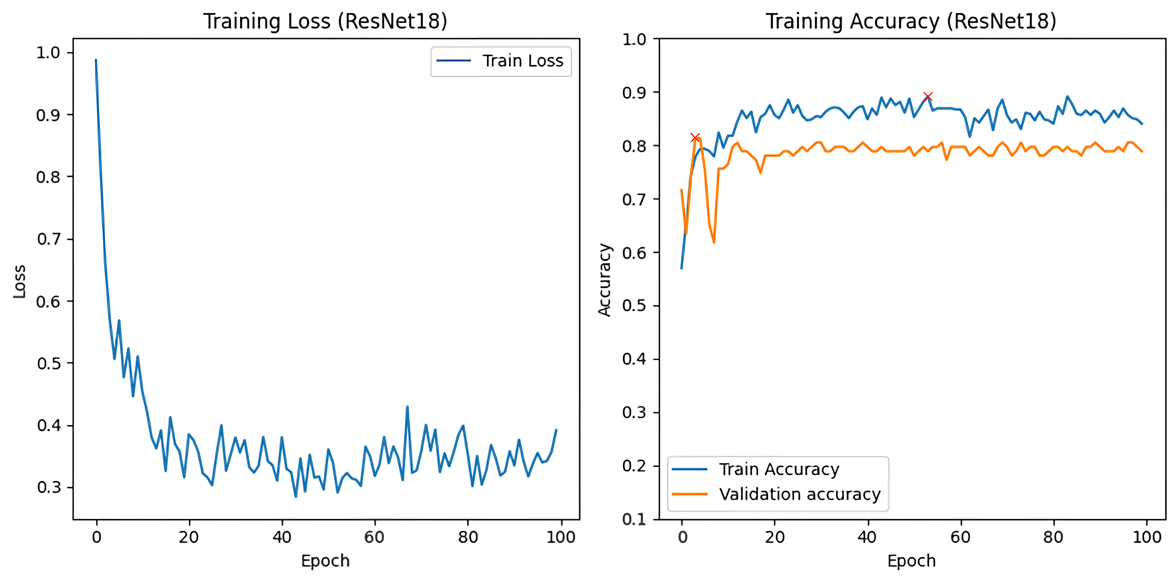
\includegraphics[height=4cm]{gambar/TrainingGraphResNet18class-weighted.png}}
	\caption{Graph of Training Loss and Accuracy from ResNet-18 With Class-weight Adjustment}
	\label{fig:graphTrainingWeightedPt1}
\end{figure}
\begin{figure}[hbtp]
	{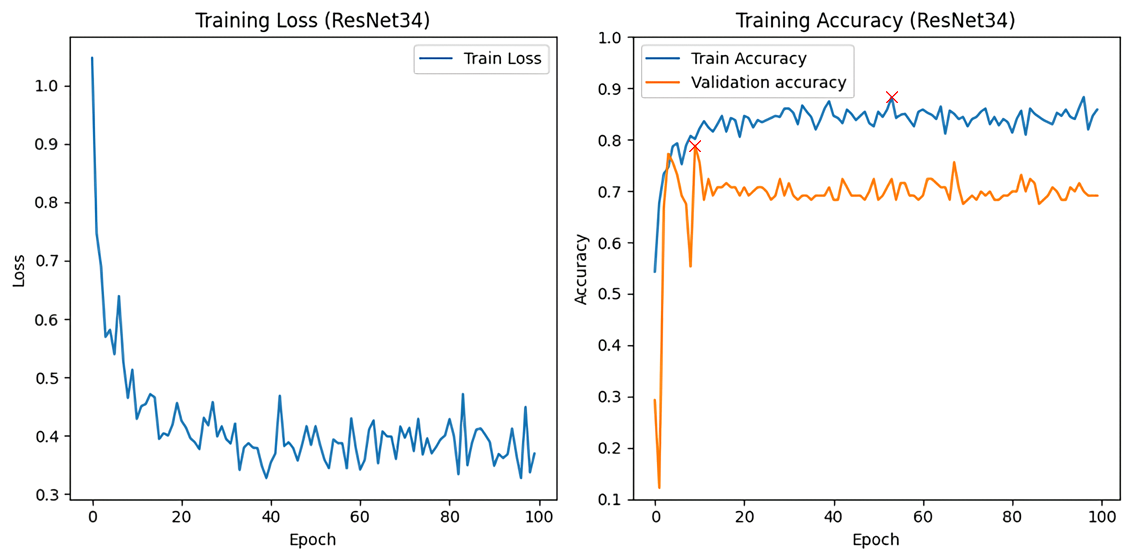
\includegraphics[height=4cm]{gambar/TrainingGraphResNet34class-weighted.png}}
	\caption{Graph of Training Loss and Accuracy from ResNet-34 With Class-weight Adjustment}
	\label{fig:graphTrainingWeightedPt2}
\end{figure}
\begin{figure}[hbtp]
	\centering
	{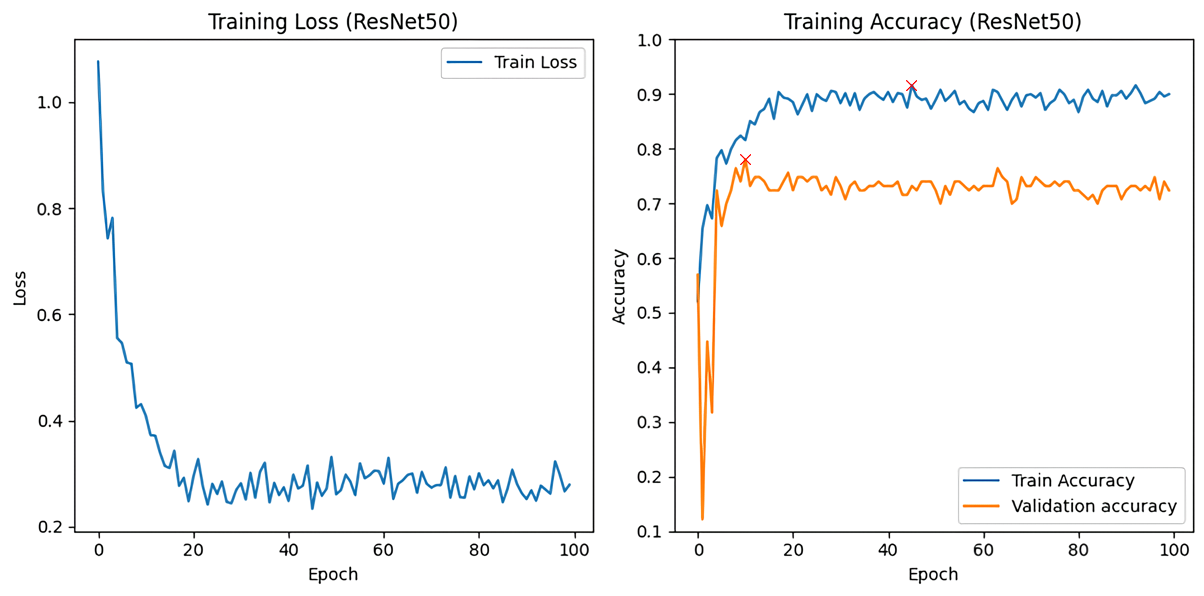
\includegraphics[height=4cm]{gambar/TrainingGraphResNet50class-weighted.png}}
	\caption{Graph of Training Loss and Accuracy from ResNet-50 With Class-weight Adjustment}
	\label{fig:graphTrainingWeightedPt3}
\end{figure}
\begin{figure}[hbtp]
	{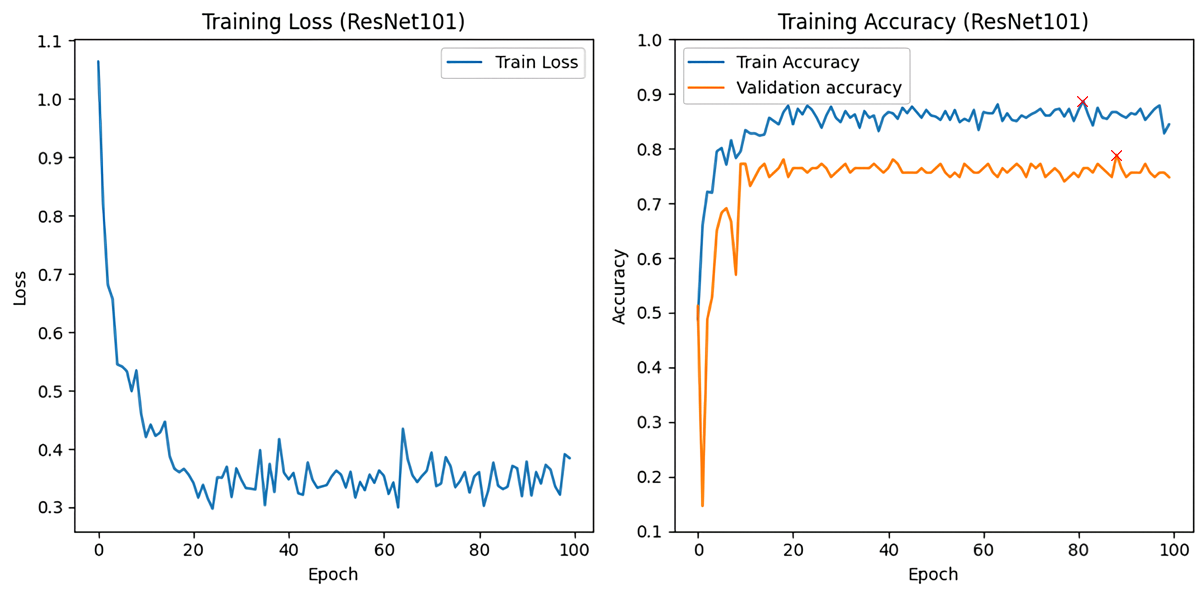
\includegraphics[height=4cm]{gambar/TrainingGraphResNet101class-weighted.png}}
	\caption{Graph of Training Loss and Accuracy from ResNet-101 With Class-weight Adjustment}
	\label{fig:graphTrainingWeightedPt4}
\end{figure}
\begin{figure}[hbtp]
	\centering
	{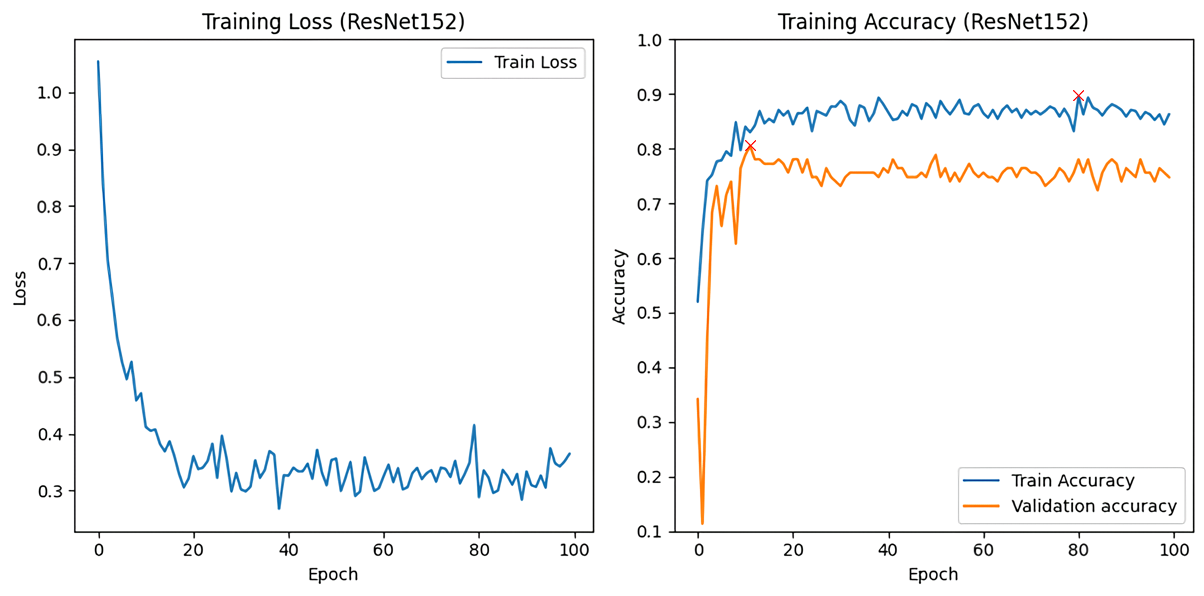
\includegraphics[height=4cm]{gambar/TrainingGraphResNet152class-weighted.png}}
	\caption{Graph of Training Loss and Accuracy from ResNet-152 With Class-weight Adjustment}
	\label{fig:graphTrainingWeightedPt5}
\end{figure}

\begin{table}[hbtp]
	\begin{center}
	\caption{Comparison of accuracy, recall on PDR class, and QWK of each best trained model with class weighting and without class weighting.}
	\label{tb:PerbandinganHasilBestTrain}
        \resizebox{\linewidth}{!}{%
    	\begin{tabular}{|c|c|lll|ccc|}
    		\hline
    		\cellcolor[HTML]{C0C0C0}                             & \cellcolor[HTML]{C0C0C0}                                  & \multicolumn{3}{c|}{\cellcolor[HTML]{C0C0C0}Akurasi Metrik}                           & \multicolumn{3}{c|}{\cellcolor[HTML]{C0C0C0}Selisih}                                                                            \\ \cline{3-8} 
    		\multirow{-2}{*}{\cellcolor[HTML]{C0C0C0}Arsitektur} & \multirow{-2}{*}{\cellcolor[HTML]{C0C0C0}Metode training} & \multicolumn{1}{c|}{Overall} & \multicolumn{1}{c|}{PDR}    & \multicolumn{1}{c|}{QWK} & \multicolumn{1}{c|}{Overall}                   & \multicolumn{1}{c|}{PDR}                        & QWK                          \\ \hline
    															 & Default                                                   & \multicolumn{1}{l|}{0,7642}  & \multicolumn{1}{l|}{0,5}    & 0,7584                   & \multicolumn{1}{c|}{}                          & \multicolumn{1}{c|}{}                           &                              \\ \cline{2-5}
    		\multirow{-2}{*}{ResNet-18}                          & \multicolumn{1}{l|}{Class-Weighted}                       & \multicolumn{1}{l|}{0,7886}  & \multicolumn{1}{l|}{0,7143} & 0,7527                   & \multicolumn{1}{c|}{\multirow{-2}{*}{0,0244}}  & \multicolumn{1}{c|}{\multirow{-2}{*}{0,214286}} & \multirow{-2}{*}{-0,005667}  \\ \hline
    															 & Default                                                   & \multicolumn{1}{l|}{0,748}   & \multicolumn{1}{l|}{0,5714} & 0,7218                   & \multicolumn{1}{c|}{}                          & \multicolumn{1}{c|}{}                           &                              \\ \cline{2-5}
    		\multirow{-2}{*}{ResNet-34}                          & \multicolumn{1}{l|}{Class-Weighted}                       & \multicolumn{1}{l|}{0,7236}  & \multicolumn{1}{l|}{0,7143} & 0,7344                   & \multicolumn{1}{c|}{\multirow{-2}{*}{-0,0244}} & \multicolumn{1}{c|}{\multirow{-2}{*}{0,142857}} & \multirow{-2}{*}{0,01261157} \\ \hline
    															 & Default                                                   & \multicolumn{1}{l|}{0,7805}  & \multicolumn{1}{l|}{0,5714} & 0,7266                   & \multicolumn{1}{c|}{}                          & \multicolumn{1}{c|}{}                           &                              \\ \cline{2-5}
    		\multirow{-2}{*}{ResNet-50}                          & \multicolumn{1}{l|}{Class-Weighted}                       & \multicolumn{1}{l|}{0,7317}  & \multicolumn{1}{l|}{0,5714} & 0,7416                   & \multicolumn{1}{c|}{\multirow{-2}{*}{-0,0488}} & \multicolumn{1}{c|}{\multirow{-2}{*}{0}}        & \multirow{-2}{*}{0,01498176} \\ \hline
    															 & Default                                                   & \multicolumn{1}{l|}{0,7805}  & \multicolumn{1}{l|}{0,7143} & 0,7504                   & \multicolumn{1}{c|}{}                          & \multicolumn{1}{c|}{}                           &                              \\ \cline{2-5}
    		\multirow{-2}{*}{ResNet-101}                         & \multicolumn{1}{l|}{Class-Weighted}                       & \multicolumn{1}{l|}{0,7642}  & \multicolumn{1}{l|}{0,7857} & 0,7133                   & \multicolumn{1}{c|}{\multirow{-2}{*}{-0,0163}} & \multicolumn{1}{c|}{\multirow{-2}{*}{0,071428}} & \multirow{-2}{*}{-0,0370362} \\ \hline
    															 & Default                                                   & \multicolumn{1}{l|}{0,7967}  & \multicolumn{1}{l|}{0,4286} & 0,6937                   & \multicolumn{1}{c|}{}                          & \multicolumn{1}{c|}{}                           &                              \\ \cline{2-5}
    		\multirow{-2}{*}{ResNet-152}                         & \multicolumn{1}{l|}{Class-Weighted}                       & \multicolumn{1}{l|}{0,7805}  & \multicolumn{1}{l|}{0,8571} & 0,7424                   & \multicolumn{1}{c|}{\multirow{-2}{*}{-0,0162}} & \multicolumn{1}{c|}{\multirow{-2}{*}{0,428572}} & \multirow{-2}{*}{0,04868909} \\ \hline
    		\end{tabular}
        }
	\end{center}
\end{table}

\begin{table}[hbtp]
	\begin{center}
	\caption{Comparison of Accuracy, Recall on PDR class, and QWK of each best validated model with class weighting and without class weighting.}
	\label{tb:PerbandinganHasilBestVal}
        \resizebox{\linewidth}{!}{%
    	\begin{tabular}{|c|c|lll|ccc|}
    		\hline
    		\cellcolor[HTML]{C0C0C0}                             & \cellcolor[HTML]{C0C0C0}                                  & \multicolumn{3}{c|}{\cellcolor[HTML]{C0C0C0}Akurasi Metrik}                           & \multicolumn{3}{c|}{\cellcolor[HTML]{C0C0C0}Selisih}                                                                            \\ \cline{3-8} 
    		\multirow{-2}{*}{\cellcolor[HTML]{C0C0C0}Arsitektur} & \multirow{-2}{*}{\cellcolor[HTML]{C0C0C0}Metode training} & \multicolumn{1}{c|}{Overall} & \multicolumn{1}{c|}{PDR}    & \multicolumn{1}{c|}{QWK} & \multicolumn{1}{c|}{Overall}                   & \multicolumn{1}{c|}{PDR}                        & QWK                          \\ \hline
    															 & Default                                                   & \multicolumn{1}{l|}{0,8211}  & \multicolumn{1}{l|}{0,5}    & 0,7333                   & \multicolumn{1}{c|}{}                          & \multicolumn{1}{c|}{}                           &                              \\ \cline{2-5}
    		\multirow{-2}{*}{ResNet-18}                          & \multicolumn{1}{l|}{Class-Weighted}                       & \multicolumn{1}{l|}{0,813}   & \multicolumn{1}{l|}{0,5}    & 0,6266                   & \multicolumn{1}{c|}{\multirow{-2}{*}{-0,0081}} & \multicolumn{1}{c|}{\multirow{-2}{*}{0}}        & \multirow{-2}{*}{-0,1066245} \\ \hline
    															 & Default                                                   & \multicolumn{1}{l|}{0,8049}  & \multicolumn{1}{l|}{0,5714} & 0,7074                   & \multicolumn{1}{c|}{}                          & \multicolumn{1}{c|}{}                           &                              \\ \cline{2-5}
    		\multirow{-2}{*}{ResNet-34}                          & \multicolumn{1}{l|}{Class-Weighted}                       & \multicolumn{1}{l|}{0,7886}  & \multicolumn{1}{l|}{0,8571} & 0,6915                   & \multicolumn{1}{c|}{\multirow{-2}{*}{-0,0163}} & \multicolumn{1}{c|}{\multirow{-2}{*}{0,285714}} & \multirow{-2}{*}{-0,0159034} \\ \hline
    															 & Default                                                   & \multicolumn{1}{l|}{0,7967}  & \multicolumn{1}{l|}{0,5}    & 0,7051                   & \multicolumn{1}{c|}{}                          & \multicolumn{1}{c|}{}                           &                              \\ \cline{2-5}
    		\multirow{-2}{*}{ResNet-50}                          & \multicolumn{1}{l|}{Class-Weighted}                       & \multicolumn{1}{l|}{0,7805}  & \multicolumn{1}{l|}{0,6429} & 0,7084                   & \multicolumn{1}{c|}{\multirow{-2}{*}{-0,0162}} & \multicolumn{1}{c|}{\multirow{-2}{*}{0,142857}} & \multirow{-2}{*}{0,00330785} \\ \hline
    															 & Default                                                   & \multicolumn{1}{l|}{0,8049}  & \multicolumn{1}{l|}{0,5}    & 0,6899                   & \multicolumn{1}{c|}{}                          & \multicolumn{1}{c|}{}                           &                              \\ \cline{2-5}
    		\multirow{-2}{*}{ResNet-101}                         & \multicolumn{1}{l|}{Class-Weighted}                       & \multicolumn{1}{l|}{0,7886}  & \multicolumn{1}{l|}{0,7857} & 0,7077                   & \multicolumn{1}{c|}{\multirow{-2}{*}{-0,0163}} & \multicolumn{1}{c|}{\multirow{-2}{*}{0,285714}} & \multirow{-2}{*}{0,01771292} \\ \hline
    															 & Default                                                   & \multicolumn{1}{l|}{0,813}   & \multicolumn{1}{l|}{0,5}    & 0,7303                   & \multicolumn{1}{c|}{}                          & \multicolumn{1}{c|}{}                           &                              \\ \cline{2-5}
    		\multirow{-2}{*}{ResNet-152}                         & \multicolumn{1}{l|}{Class-Weighted}                       & \multicolumn{1}{l|}{0,8049}  & \multicolumn{1}{l|}{0,8571} & 0,7053                   & \multicolumn{1}{c|}{\multirow{-2}{*}{-0,0081}} & \multicolumn{1}{c|}{\multirow{-2}{*}{0,357143}} & \multirow{-2}{*}{-0,0250226} \\ \hline
    		\end{tabular}
        }
	\end{center}
\end{table}

\begin{table}[hbtp]
\begin{center}
	\caption{Comparison of accuracy, recall on PDR class, and QWK of each Last Trained Model with Class weighting and without Class weighting.}
	\label{tb:PerbandinganHasilLastTrained}
        \resizebox{\linewidth}{!}{%
    	\begin{tabular}{|c|c|lll|ccc|}
    		\hline
    		\cellcolor[HTML]{C0C0C0}                             & \cellcolor[HTML]{C0C0C0}                                  & \multicolumn{3}{c|}{\cellcolor[HTML]{C0C0C0}Akurasi Metrik}                           & \multicolumn{3}{c|}{\cellcolor[HTML]{C0C0C0}Selisih}                                                                            \\ \cline{3-8} 
    		\multirow{-2}{*}{\cellcolor[HTML]{C0C0C0}Arsitektur} & \multirow{-2}{*}{\cellcolor[HTML]{C0C0C0}Metode training} & \multicolumn{1}{c|}{Overall} & \multicolumn{1}{c|}{PDR}    & \multicolumn{1}{c|}{QWK} & \multicolumn{1}{c|}{Overall}                   & \multicolumn{1}{c|}{PDR}                        & QWK                          \\ \hline
    															 & Default                                                   & \multicolumn{1}{l|}{0,7642}  & \multicolumn{1}{l|}{0,5714} & 0,7544                   & \multicolumn{1}{c|}{}                          & \multicolumn{1}{c|}{}                           &                              \\ \cline{2-5}
    		\multirow{-2}{*}{ResNet-18}                          & \multicolumn{1}{l|}{Class-Weighted}                       & \multicolumn{1}{l|}{0,7724}  & \multicolumn{1}{l|}{0,7143} & 0,715                    & \multicolumn{1}{c|}{\multirow{-2}{*}{0,0082}}  & \multicolumn{1}{c|}{\multirow{-2}{*}{0,142857}} & \multirow{-2}{*}{-0,0393818} \\ \hline
    															 & Default                                                   & \multicolumn{1}{l|}{0,7724}  & \multicolumn{1}{l|}{0,5}    & 0,7289                   & \multicolumn{1}{c|}{}                          & \multicolumn{1}{c|}{}                           &                              \\ \cline{2-5}
    		\multirow{-2}{*}{ResNet-34}                          & \multicolumn{1}{l|}{Class-Weighted}                       & \multicolumn{1}{l|}{0,748}   & \multicolumn{1}{l|}{0,5714} & 0,7137                   & \multicolumn{1}{c|}{\multirow{-2}{*}{-0,0244}} & \multicolumn{1}{c|}{\multirow{-2}{*}{0,071429}} & \multirow{-2}{*}{-0,0151831} \\ \hline
    															 & Default                                                   & \multicolumn{1}{l|}{0,6992}  & \multicolumn{1}{l|}{0,4286} & 0,7282                   & \multicolumn{1}{c|}{}                          & \multicolumn{1}{c|}{}                           &                              \\ \cline{2-5}
    		\multirow{-2}{*}{ResNet-50}                          & \multicolumn{1}{l|}{Class-Weighted}                       & \multicolumn{1}{l|}{0,7236}  & \multicolumn{1}{l|}{0,7143} & 0,7007                   & \multicolumn{1}{c|}{\multirow{-2}{*}{0,0244}}  & \multicolumn{1}{c|}{\multirow{-2}{*}{0,285715}} & \multirow{-2}{*}{-0,0275716} \\ \hline
    															 & Default                                                   & \multicolumn{1}{l|}{0,8049}  & \multicolumn{1}{l|}{0,5}    & 0,7418                   & \multicolumn{1}{c|}{}                          & \multicolumn{1}{c|}{}                           &                              \\ \cline{2-5}
    		\multirow{-2}{*}{ResNet-101}                         & \multicolumn{1}{l|}{Class-Weighted}                       & \multicolumn{1}{l|}{0,7724}  & \multicolumn{1}{l|}{0,7143} & 0,7423                   & \multicolumn{1}{c|}{\multirow{-2}{*}{-0,0325}} & \multicolumn{1}{c|}{\multirow{-2}{*}{0,214286}} & \multirow{-2}{*}{0,00054199} \\ \hline
    															 & Default                                                   & \multicolumn{1}{l|}{0,7398}  & \multicolumn{1}{l|}{0,5}    & 0,6851                   & \multicolumn{1}{c|}{}                          & \multicolumn{1}{c|}{}                           &                              \\ \cline{2-5}
    		\multirow{-2}{*}{ResNet-152}                         & \multicolumn{1}{l|}{Class-Weighted}                       & \multicolumn{1}{l|}{0,7154}  & \multicolumn{1}{l|}{0,6429} & 0,7273                   & \multicolumn{1}{c|}{\multirow{-2}{*}{-0,0244}} & \multicolumn{1}{c|}{\multirow{-2}{*}{0,142857}} & \multirow{-2}{*}{0,04224171} \\ \hline
    	\end{tabular}
        }
\end{center}
\end{table}


